\documentclass[10pt,landscape]{article}
\usepackage{multicol}
\usepackage{calc}
\usepackage{ifthen}
\usepackage[landscape]{geometry}
\usepackage[ngerman]{babel}
\usepackage[utf8]{inputenc}
\usepackage{graphics}
\usepackage{listings}
\usepackage{verbatim}
\usepackage{tikz}
\usetikzlibrary{arrows,automata}

% This sets page margins to .5 inch if using letter paper, and to 1cm
% if using A4 paper. (This probably isn't strictly necessary.)
% If using another size paper, use default 1cm margins.
\ifthenelse{\lengthtest { \paperwidth = 11in}}
	{ \geometry{top=.5in,left=.3in,right=.5in,bottom=.5in} }
	{\ifthenelse{ \lengthtest{ \paperwidth = 297mm}}
		{\geometry{top=1cm,left=1cm,right=1cm,bottom=1cm} }
		{\geometry{top=1cm,left=1cm,right=1cm,bottom=1cm} }
	}

% Turn off header and footer
\pagestyle{empty}
 

% Redefine section commands to use less space
\makeatletter
\renewcommand{\section}{\@startsection{section}{1}{0mm}%
                                {-1ex plus -.5ex minus -.2ex}%
                                {0.5ex plus .2ex}%x
                                {\normalfont\large\bfseries}}
\renewcommand{\subsection}{\@startsection{subsection}{2}{0mm}%
                                {-1explus -.5ex minus -.2ex}%
                                {0.5ex plus .2ex}%
                                {\normalfont\normalsize\bfseries}}
\renewcommand{\subsubsection}{\@startsection{subsubsection}{3}{0mm}%
                                {-1ex plus -.5ex minus -.2ex}%
                                {1ex plus .2ex}%
                                {\normalfont\small\bfseries}}
% Special commands
\newcommand{\code}[1]{\texttt{#1}}

\makeatother

% Define BibTeX command
\def\BibTeX{{\rm B\kern-.05em{\sc i\kern-.025em b}\kern-.08em
    T\kern-.1667em\lower.7ex\hbox{E}\kern-.125emX}}

% Don't print section numbers
\setcounter{secnumdepth}{0}


\setlength{\parindent}{0pt}
\setlength{\parskip}{0pt plus 0.5ex}


% -----------------------------------------------------------------------

\begin{document}

\raggedright
\footnotesize
\begin{multicols}{3}


% multicol parameters
% These lengths are set only within the two main columns
%\setlength{\columnseprule}{0.25pt}
\setlength{\premulticols}{1pt}
\setlength{\postmulticols}{1pt}
\setlength{\multicolsep}{1pt}
\setlength{\columnsep}{2pt}

\begin{center}
     \Large{\textbf{MuMeTech-CheatSheet}} \\
\end{center}

\section{Definition}
\subsection{MuMeTech} ist rechnergef\"uhrt, unabh\"angig, diskret und kontinuierlich.\\
\subsection{Kompression}
Daten/Datenkan\"ale werden auf bestimmte Aufl\"osung/Genauigkeit/Abtastrate reduziert (Bei unterschiedlicher Reduzierung je nach Kanal, nennt man es Subsampling).
\subsection{\"Ubertragungsmodi}
\begin{itemize}
    \item \textbf{synchron} Der Sender sendet direkt an den Empf\"anger, es kann erst weitergesendert werden, wenn die Daten empfangen werden. (Handy)
    \item \textbf{asynchron} Die Daten werden w\"ahrend der \"Ubertragung zwischengepuffert, womit der Sender nicht auf den Empf\"anger warten muss. (Post,EMail)
    \item \textbf{isochron} Zeitraster ist fest, konstante Periode und Datenrate. (USB)
\end{itemize}

\subsection{Medienarten}
\begin{itemize}
    \item \textbf{Perzeptionsm.} Wahrnehmung
    \item \textbf{Repr\"asentationsm.} Darstellung
    \item \textbf{Pr\"asentationsmedium} Ausgabe
    \item \textbf{Speichermedium} Physikalischer Datenspeicher
\end{itemize}

\section{Kompressionsarten}
\subsection{Huffmann} \ \\
H\"aufige Zeichen $\Rightarrow$ kurze Codew\"orter\\
Weniger h\"aufige Zeichen $\Rightarrow$ lange Codew\"orter \\
Zeichen werden nach ihrer H\"aufigkeit geordnet mit verschieden langen Codes repr\"asentiert.
\subsubsection{Beispiel nach Sonny}
\paragraph{Schritt 1} \ \\
\begin{tikzpicture}[shorten >=0.7pt,node distance=1.6cm,auto]
    \node[state]  (b) [label=above:$2$]                    {b};
    \node[state]  (a) [right of=b,label=above:$3$]         {a};
    \node[state]  (d) [right of=a,label=above:$3$]         {d};
    \node[state]  (e) [right of=d,label=above:$4$]         {e};
    \node[state]  (c) [right of=e,label=above:$6$]         {c};
\end{tikzpicture}
\paragraph{Schritt 2} \ \\
\begin{tikzpicture}[shorten >=0.7pt,node distance=1.6cm,auto]
    \node[state]  (d) [label=above:$3$]                     {d};
    \node[state]  (e) [right of=d,label=above:$4$]          {e};
    \node[state]  (5) [right of=e]                          {5};
    \node[state]  (c) [right of=5,label=above:$6$]          {c};
    \node[state]  (b) [below left of=5,label=above:$2$]     {b};
    \node[state]  (a) [below right of=5,label=above:$3$]    {a};
    \path[->]   (5)     edge  node {} (a)
                (5)     edge  node {} (b)
                ;
\end{tikzpicture}
\paragraph{Schritt 3} \ \\
\begin{tikzpicture}[shorten >=0.7pt,node distance=1.6cm,auto]
    \node[state]  (5)                           {5};
    \node[state]  (c) [right of=5,label=above:$6$]          {c};
    \node[state]  (b) [below left of=5,label=above:$2$]     {b};
    \node[state]  (a) [below right of=5,label=above:$3$]    {a};
    \node[state]  (7) [right of=c]                          {7};
    \node[state]  (d) [below left of=7,label=above:$3$]     {d};
    \node[state]  (e) [below right of=7,label=above:$4$]     {e};

    \path[->]   (5)     edge  node {} (a)
                (5)     edge  node {} (b)
                (7)     edge  node {} (d)
                (7)     edge  node {} (e)
                ;
\end{tikzpicture}

\paragraph{Schritt 4} \ \\
\begin{tikzpicture}[shorten >=1pt,node distance=2cm,auto]
    \node[state]  (7) []                                    {7};
    \node[state]  (d) [below left of=7,label=above:$3$]     {d};
    \node[state]  (e) [below right of=7,label=above:$4$]    {e};
    \node[state]  (11) [right of=7]                         {11};
    \node[state]  (5) [below right of=11]                   {5};
    \node[state]  (c) [below left of=11,label=above:$6$]    {c};
    \node[state]  (b) [below left of=5,label=above:$2$]     {b};
    \node[state]  (a) [below right of=5,label=above:$3$]    {a};
    
    \path[->]   (5)     edge  node {} (a)
                (5)     edge  node {} (b)
                (7)     edge  node {} (d)
                (7)     edge  node {} (e)
                (11)     edge  node {} (c)
                (11)     edge  node {} (5)
                ;
\end{tikzpicture}

\paragraph{Schritt 5} \ \\
\begin{tikzpicture}[shorten >=1pt,node distance=1.6cm,auto]
    \node[state]  (18) []                                    {18};
    \node[state]  (7)  [below left of=18]                    {7};
    \node[state]  (d)  [below left of=7,label=above:$3$]     {d};
    \node[state]  (e)  [below right of=7,label=above:$4$]    {e};
    \node[state]  (11) [below right of=18]                         {11};
    \node[state]  (5)  [below right of=11]                   {5};
    \node[state]  (c)  [below left of=11,label=above:$6$]    {c};
    \node[state]  (b)  [below left of=5,label=above:$2$]     {b};
    \node[state]  (a)  [below right of=5,label=above:$3$]    {a};
    
    \path[->]   (5)     edge  node {} (a)
                (5)     edge  node {} (b)
                (7)     edge  node {} (d)
                (7)     edge  node {} (e)
                (11)     edge  node {} (c)
                (11)     edge  node {} (5)
                (18)     edge  node {} (7)
                (18)     edge  node {} (11)
                ;
\end{tikzpicture}

\paragraph{Schritt 5} \ \\
\begin{tikzpicture}[shorten >=1pt,node distance=1.6cm,auto]
    \node[state]  (18) []                                    {18};
    \node[state]  (7)  [below left of=18]                    {7};
    \node[state]  (d)  [below left of=7,label=below:$3$]     {d};
    \node[state]  (e)  [below right of=7,label=below:$4$]    {e};
    \node[state]  (11) [below right of=18]                         {11};
    \node[state]  (5)  [below right of=11]                   {5};
    \node[state]  (c)  [below left of=11,label=below:$6$]    {c};
    \node[state]  (b)  [below left of=5,label=below:$2$]     {b};
    \node[state]  (a)  [below right of=5,label=below:$3$]    {a};
    
    \path[->]   (5)     edge  node {1} (a)
                (5)     edge  node {0} (b)
                (7)     edge  node {1} (d)
                (7)     edge  node {0} (e)
                (11)     edge  node {0} (c)
                (11)     edge  node {1} (5)
                (18)     edge  node {0} (7)
                (18)     edge  node {1} (11)
                ;
\end{tikzpicture}
$\Rightarrow$ \\
d: 00\\
e: 01\\
b: 100\\
a: 101\\
c: 11\\
Mittlere Codel\"ange (Kompressionsfaktor): 41/18


\subsection{Laufl\"angenkodierung}
Fasst direkt aufeinanderfolgende Zeichenketten zusammen. ($aaabbb \Rightarrow 3a3b$)

\section{Erdn\"usse}
\subsection{FFT}
Spaltet komplexes Signal in mehrere reine Sinusschwingungen auf, welche addiert das Orginalsignal ergeben.
\subsection{DCT}
Wichtige Elemente der darzustellenden Daten werden mit mehr Bandbreite versehen (Links-Oben-Bild) \\
\textbf{Die DCT ist verlustfrei umkehrbar-Erst durch die Quantisierung findet die Reduktion statt.}

\section{Audio}
\subsection{Begriffe}
\begin{itemize}
    \item \textbf{Phon} Empfundene Lautst\"arke im Verh\"altnis zu 1000 Hz Sinus. Skaliert normal (nicht log.).
    \item \textbf{Dezibel} Logarithmisch ausgedr\"uckte Lautst\"arke 6dB Unterschied bedeuten Verdoppelung der Lautst\"arke.
    \item \textbf{Frequenzamplitude} Amplitude wird angegeben in Dezibel und bestimmt die Lautst\"arke. Beschreibt maximale Auslenkung der Sinuswelle.
    \item \textbf{Klang} Schallwelle die vom menschlichen Ohr als bestimmter Ton wahrgenommen wird.
\end{itemize}
\subsection{Analog2Digital}
\begin{enumerate}
    \item \textbf{Vorverarbeitung} Filterung (St\"orger\"ausche), Verst\"arkung (Dynamikausnutzung) \\
    Im zweiten Schritt erfolgt eine Frequenzbandbegrenzung (Tiefpassfilter) auf $1/2$ der Abtastfrequenz (Shannon Abtasttherorem)
    \item \textbf{Abtastung} In konstanten Intervallen wird der Wert des Eingangssignals entnommen.
    \item \textbf{Quantisierung} Diskretisierung des bei der Abtastung ermittelten Wertes 
    \item \textbf{Kodierung} Bin\"arkodierung der Signalproben
\end{enumerate}
\textbf{Zusammenfassend} \\
Aus einem zeitkontinuierlich ablaufendem VOrgang werden Signalproben genommen und in ihrer Amplitude quantisiert und in eine computergerechte Darstellung gebracht.

\subsection{Kodierungsmethoden}
\textbf{Verlustbehaftet}
\begin{itemize}
    \item \textbf{PulseCodeModulation - PCM} 3 Schritte \\
        \begin{itemize}
        \item \textbf{Schritt 1} Abtastung mit zeitlich konst. Rate
        \item \textbf{Schritt 2} Quantisierung der Werte
        \item \textbf{Schritt 3} Kodierung in bin\"arcode \\
            Die Kodierung erfolt linear. 
        \end{itemize}
    \item \textbf{DPCM} Differenzielle PCM \\
        Die Quantisierung erfolgt anhand der Differenz zu einer Vorhersage. \\
        \textbf{Bei DPCM werden Differenzwerte aufeinanderfolgender Abtastwerte gebildet.}
    \item \textbf{DeltaModulation} Eine DPCM mit nur einem Bit. Wertebereich -/+1.
    Die Sch\"atzwerte nehmen dabei immer an, dass der neue Abtastwert gleich dem vorherigem ist.
    \item \textbf{Adaptive differenzielle PCM} \"Ahnlich DPCM, jedoch mit dyamischer Vorhersage.
     Angepasste Quantisierung, dadurch bessere Quali.
\end{itemize}
\subsection{Kompressionsverfahren f\"ur Audio}
\subsubsection{Datenreduktion}
Filterung der Daten (z.B. nach psychoakustik).
\subsubsection{Datenkompression}
Verlustfreie Komprimierung der Daten.

\subsection{mp3}
\begin{enumerate}
    \item PCM (768Kbit/s)
    \item Filterbank f\"ur 32 Subb\"ander / FastFourierTrans f\"ur 1024 Abtastwerte
    \item FFT $\Rightarrow$ PsychAkModel nun wird anhand derer und der Subb\"ander quantisiert.
    \item Audiodatenkodierung mit Huffmann, Nebeninfos codiert
    \item BitstromFormatierung und Fehlerkorrektur
\end{enumerate}

\subsection{MIDI}
Daten\"ubertragungsprotokoll f\"ur Musikdaten.\"Ubertragen werden Steuerinformationen zwischen elektronischen Instrumenten, welche von Programm interpretiert werden k\"onnen. \\
Inhalt zum Beispiel: Anschlagst\"arke, Lautst\"arke, MidiKanalnummer (4Bit), Spurname \\
\begin{itemize}
    \item[Format 0] Alle Midikan\"ale sind in einer Spur zusammengefasst, somit keine gleichzeitigen Anschl\"age verschiedener Instrumente (Klingelton) 
    \item[Format 1] Jeder Kanal hat eigene Spur, somit k\"onnen auch gleichzeitige Anschl\"age realisiert werden.
    \item[Format 2] Im Format 2 besteht jede Spur (Track) aus unabh\"angigen Einheiten. Im Gegensatz zu SMF 1 k\"onnen also mehrere Spuren dieselbe MIDI-Kanal-Nummer haben.
\end{itemize}
\textbf{THRU-Port} gibt parallel zum Outport eines Ger\"ates (z.B. Filter) das unbehandelte Inputsignal aus (z.B. f\"ur Aufnahmen).

\subsection{Beispielrechnungen}
\textbf{Einheiten:} \\
$1MB \Rightarrow 10^6 Byte || 1MiB \Rightarrow 1024 \times 1024 Byte$ \\
$1GB \Rightarrow 10^9 Byte || 1GiB \Rightarrow 1024 \times 1024 \times 1024 Byte$ \\
\subsubsection{PCM: 44.1KHz,16Bit,stereo,20min}
$44.100 \times 16 \times 2 \times 20 \times 60 \Rightarrow Bit$ \\
$44.100 \times 2 \times 2 \times 20 \times 60 \Rightarrow 211680000 Byte \approx 211.7 MB$ \\
\subsubsection{MP3: 128kbit/s}


\section{Grafiken/Bilder}
\subsection{Farbmodi}
\begin{itemize}
    \item \textbf{RGB} RotGr\"unBlau.\\
        Additive Farbmischung mit drei Farbkan\"ale a 8Bit (default).
        \begin{itemize}
            \item \textbf{Anwendungen} Monitordarstellung, Kamera
            \item \textbf{Vorteile} \\
                Gut auf Ger\"aten anzuwenden, die Lichtquellen aussenden.\\
                Direkt mit Algo bearbeitbar\\
                Darstellungskapazit\"at vieler Farbnuancen
            \item \textbf{Nachteil} \\
                Probleme mit Darstellung von Schwarz \\
                Ger\"ateabh\"angig. \\
                8 \% des Farbraums sind nicht wahrnehmbare Farben \\
                Helligkeitskorrektur schwer \\
                Eignet sich nicht f\"ur Druck (Additiv/Substraktiv)
        \end{itemize}
    \item \textbf{YUV}
        Darstellung durch Luminanz (Y) und Chrominanz (UV).
        \begin{itemize}
            \item \textbf{Anwendungen} Analoges NTSC/PAL-Farbfernsehen
            \item \textbf{Vorteile} \\
                Halbe Bandbreite von RGB \\
                Durch Subsampling optimierung m\"oglich (siehe Subsampling)\\
                Vollst\"andiger Farbraum abgedeckt\\
                Abw\"artskompatibel zu Schwarz/Weiss\\
                Ausnutzung Wahrnehmungspsychologie\\
                Helligkeit separat im Gegensatz zu RGB (jeder Kanal muss angepasst werden)\\
                Progressive Vollbilder m\"oglich
            \item \textbf{Nachteil} \\
                Verteilung der Farbanteile der Cyan/Orange und Megenta/Gr\"un ist ungleichm\"assig auf U und V, daher keine Bandbreitenreduktion m\"oglich
        \end{itemize}
    \item \textbf{YIQ}
        Darstellung durch Luminanz (Y), sowie den Farbdifferenzen I (Cyan/Orange) und Q (Magenta/Gr\"un) \\
        Irgendwie zu YUV verdreht! WHY? How much?
        \begin{itemize}
            \item \textbf{Anwendungen} Altes analoges NTSC-Farbfernsehen 
            \item \textbf{Vorteile} \\
                \"Ahnlich YUV \\
                Kommt wahrscheinlich nicht in der Klausur dran (Jonas)
            \item \textbf{Nachteil} \\
                Nur \"uberm Teich im Gebrauch
        \end{itemize}
\end{itemize}

\subsection{JPEG}
\subsubsection{JPEG-Kodierung}
\textbf{Subsampling (verlustbehaftet und verlustfrei, z.B. ist 4:4:4 verlustfrei), DCT auch verlustfrei, Quantisierung bringt Datenreduktion (nicht verlustfrei umkehrbar)}
\begin{itemize}
    \item \textbf{Bildvorverarbeitung (verlustfrei)}
        \begin{itemize}
            \item Grauwerttransformation (Kontrasterh\"ohung und Helligkeitsverbesserung)
            \item Bildfilterung (Rauschunterdr\"uckung,Kantenverst\"arkung,Gl\"attung,...)
        \end{itemize}
    \item \textbf{Bildverarbeitung (theo. verlustfrei)}
    \begin{itemize}
        \item Abtastung und Digitaliserung der Bildinformationen.
        \item Einteilung in 8x8-Pixel-Bl\"ocke, wobei jeder Pixel mit 8bit kodiert wird (optimaler Kompromis zwischen Laufzeit und Quali; Zahl f\"ur DCT).
        \item DCT Der 8Bit-Farbwert wird vom Ortsbereich- in den Frequenzbereich transformiert. \\
            Das Ergebnis ist eine 8x8-Frequenzraummatrix S, $S_{00}$ entspricht dem Anteil der Freuqenz 0 (Grundfarbton), dieser ist der DC-Koeffizient.\\
            Alle anderen $S_{ij}$ heissen AC-Koeffizienten und geben Auskunft \"uber die Frequenzver\"anderungen (Farbver.) innerhalb des Blockes.\\
            Der letzte Eintrag $S_{77}$ gibt dabei die h\"ochste in beiden Richtungen auftretene Frequenz an.
    \end{itemize}
    \item \textbf{Quantisierung (verlustbehaftet)} Erstellen einer ZickZack-Sequenz (Diagonaler Schnitt von links-oben an). Ausnutzung des PsychoVisuellenModels (PVM).
        Die Anwendung stellt eine Liste mit 64 Faktoren zur Verf\"ugung. Anhand dieser werden die DCT-Koeffizienten gewichtet (und gerundet),
        wodurch die Freuqenzwechsel an die Qualit\"atsanforderung angepasst werden.\\
        Wird die Qualit\"at reduziert, so ist die rechte untere Dreiecksmatrix mit Nullen versehen. Dies kommt der Entropiekodierung zu Gute.
    \item \textbf{Entropiekodierung (verlustfrei)} Die resultierdende Liste wird mit Huffmann oder aritmetisch kodiert.    
\end{itemize}
\subsubsection{JPEG-Modi}
\begin{itemize}
    \item \textbf{Sequenzielle mode} Das Bild wir din einem einzigen Durchlauf kodiert.
    \item \textbf{progressive mode} Das Bild wird in mehreren Durchl\"aufen immer genauer kodiert.\\
        Vorteil: Schnelle (grobpixelige) Vorschau des Bildes
    \item \textbf{Hirachischer Modus} Das Bild wird in verschiedenen Aufl\"osungen kodiert.\\
        Vorteil: Jede Anwendung greift sich ihre geeignete Aufl\"osung heraus und muss nicht rekodieren.
    \item \textbf{lossless mode} Verlustfreie Kodierung des Bildes
\end{itemize}

\section{Netzwerk/Internet}
\subsection{IP-Adresse/Subnetzmaske}
IP-Adresse wird zur genauen Identifikation eines Host genutzt und besteht aus 32Bit.\\
Sie wird in ClassA-D eingeteilt. Hierzu wird die IP mit der Subnetzmaske AND-Verkn\"upft, das Ergebnis ist die NetzID. \\
Eine ClassX-Subnetzmaske besteht aus f\"uhrenden Einsen, gefolgt von Nullen. Abk\"urzend wird nur die Anzahl der Einsen angegeben:
\subsubsection{192.168.1.23/24 (SM: 255.255.255.0)}
$11000000.10101000.00000001.00010111$ (IP-Adresse)\\
$11111111.11111111.11111111.00000000$ (Subnetzmaske)\\
$11000000.10101000.00000001.00000000 \Rightarrow$ (NetzwerkID)\\
$00000000.00000000.00000000.00010111 \Rightarrow$ (HostID)\\
\subsubsection{Subnetting}
Um die z.T. riesigen Netze logisch zu unterteilen, kann von der ClassA-D Begrenzung abgewichen werden, \\
daraus ergeben sich dann kleine Teilnetze.
\begin{itemize}
    \item \textbf{Vorteil} \\
        - Durch kleine Subnetze wirken sich z.B. Broadcasts nicht auf das Riesennetz aus.\\
        - Hostgruppen k\"onnen getrennt werden.
    \item \textbf{Nachteil} Kompromiss: \\
    'grosses Netz mit Broadcast-Probleme' vs 'kleine Netze die mit Router verbunden werden m\"ussen'
\end{itemize}
\begin{verbatim}
                                Adressen
123.45.64.0/18      - Provider  16384
  123.45.64.0/20    - Kunde A   4096
    123.45.64.0/28  - A1        16
    123.45.64.16/28 - A2        16
  123.45.80.0/20    - Kunde B   4096
123.45.96.0/19      - Kunde C   8192
\end{verbatim}

\subsection{\"Ubertragungsarten}
\begin{itemize}
    \item \textbf{unicast (1:1)} Normale Netzwerkverbindung z.B. Client/Server (Mail, http)
    \item \textbf{broadcast (1:n)} Ein Host kommuniziert mit allen Knoten im Netzwerk (Subnetz), zB. um einen DHCP-Server zu finden 
    \item \textbf{multicast (1:m)} Ein Host sendet Daten an mehrere Empf\"anger (z.B. Videostream), die Bandbreite erh\"oht sich nicht mit der Anzahl der Empf\"anger. 
    \item \textbf{multipeer (m:m)} Mehrere Hosts senden und empfangen gleichberechtigt in einer Hostgruppe. (z.B. Videokonferenz)
\end{itemize}

\subsection{AJAX}
Dient dem Asynchronen Datenaustausch um Inhalte dynamisch nachzuladen. Dabei muss stets nur das Frame der Webseite nachgeladen werden, welches ver\"andert wird.\\
\begin{itemize}
    \item \textbf{Voraussetzungen} JavaScript, XML-HTTP-Request. Zur Darstellung wird HTML,JavaScript und DOM genutzt.
    \item \textbf{Vorteile} \\
    - Daten k\o"nnen ver\"andert werden, ohne die Seite komplett laden zu m\"ussen.\\
    - Webanwendungen k\"onnen schneller auf Benutzereingaben reagieren.\\
    - Kein unn\"otiges Nachladen von statischen Inhalten\\
    - AJAX schafft ein desktopähnliches Verhalten einer Web-App
    \item \textbf{Nachteil}\\
    - Abh\"angigkeit von JavaScript (5\% der User haben es nicht aktiviert)\\
    - Vor-/Zur\"uckbutton des Browsers nicht mehr funktionst\"uchtig, da Browser i.d.R. nur die statischen Daten speichern\\
    - Lesezeichen setzen, etc. nicht mehr m\"oglich\\
    - Testing der Anwendung aufwendig\\
    - Die Latenzzeit des Server kann nachteilig wirken (hohe Serverlast$\rightarrow$Unzufriedenheit des Users)
\end{itemize}

\subsection{HTML5}
Liste von neuen Tags:
\begin{itemize}
    \item \textbf{audio} Definiert Audioinhalte
    \item \textbf{video} Definiert Videoinhalte
    \item \textbf{time} Datumsdefinitions
    \item \textbf{article} Artikel
    \item \textbf{canvas}  2D-Bitmap-Zeichenfl\"ache
    \item \textbf{details} Detailinformationen zu einem Element
    \item \textbf{section} Erleichtert das Abgrenzen von unterschiedlichen Inhalten, soll das div-Tag ersetzen
\end{itemize}
Weiter wurde der DOCTYPE in HTML5 auf einen HTML-Typen zusammengestrichen, HTML4 kennt noch drei Doctypes.\\
Die Sprache befindet sich z.Zt. noch in der Entwicklung (MARCO).

\subsection{HTTP}
\"Ubermittlungsprotokoll f\"ur das WWW, erfunden 1995 von Tim Berners Lee am CERN in Genf.
\begin{verbatim}
TCP-Verbindungsaufbau (Handshake)
-> GET http://URL (Client fordert Inhalt an)
<- HTTP/1.X 200 OK (Response von Server)
\end{verbatim}

\section{MPEG}
\subsection{MPEG1}
\subsubsection{Subsection}
Dient zur Speicherreduktion indem Chrominanz im Vergleich zur Luminanz mit veringerter Abtastrate gespeichert wird (PAVM),
da Helligkeit- besser als Farbunterschiede wahrgenommen werden.\\

\subsubsection{Subsampling}
\begin{itemize}
    \item 4:4:4 (MPEG1 verwendet) \\   
        Unkomprimiert, Farb und Helligkeitsinformationen werden gleich haeufig abgetastet.
    \item 4:2:2
        Abtastrate der Farbkanaele in horizontaler Richtung halb so gross wie in vertikalter Richtung.
        Anwendung beim Analog-Farbsehen wegen dem Zeilensprungverfahren.
    \item 4:2:0
        Wird bei digitalen Bildern wie JPEG und MPEG angewedet.
        Abtastung in beide Richtungen identisch.
\end{itemize}

\subsection{Kodierung}
\begin{itemize}
    \item \textbf{1. Schritt:} Bildaufbereitung: Konversion der Farbraums (von 24 Bit RGB in Y,Cr,Cb), Anwendung der Kodierung
    \item \textbf{2. Schritt:} 4.2.2 Subsampling
    \item \textbf{3. Schritt:} Einteilung in Makro-Bloecke
    \item \textbf{4. Schritt:} Bewegungsvorhersagealgorithmus: Vgl des aktuellen Makro-Blocks mit den umgebenden und den Makro-Bloecken des vor- und nachfolgenden Einzelbilds. Aehnlich wie bei der DPCM wird nur die Differenzinformation gespeichert und der Vektor kodiert.
    \item \textbf{5.Schritt:} DCT
    \item \textbf{6. Schritt:} Bildverarbeitung: Kodierung (des Videostroms)
    \item \textbf{6.1. verschieden Arten von Einzelbildern (Frames):}
    \begin{itemize}
        \item \textbf{6.1.1. I-Frame (Intracoded Picture):}
            Standbild JPEG-aehnlich ohne zusaetzliche Infos. (Kompression gering, wie bei JPEG, jedoch in Echtzeit)
        \item \textbf{6.1.2. P-Frame (Predictive Coded Picture):}
            Bezieht sich auf das vorhergehende I- oder P-Frame, enthaelt Vektoren und Bilddifferenzinformationen. (Groessere Kompr. als bei I)
        \item \textbf{6.1.3. B-Frame (Bidirectional Coded Picture):}
            Vergleicht folgendes (I- oder P-Frame) mit vorangehendem (I- oder P-)Frame und stellt Durchschnittswert dar. (Groesste Kompression)
        \item \textbf{6.1.4. D-Frame (Direct Coded Picture):}
            Bei geeigneter Speicherung der I-Frame ueberfluessig. Nur DC-Koeffizienten werden kodiert, daher schlechte Qualitaet.\\
            Nur ein Farbwert pro 8x8 Block wird gespeichert, Verwendung fuer schnellen Vorlauf.
        \item \textbf{7.Schritt:} Quantisierung: verlustbehaftet\\
            Fuer I-Frame gleich wie bei JPEG, bei P- und B-Frames werden nur die DCT-kodierten Anteile quantisiert.\\
            Bewegunsvektoren fuer P- und B-Frames werden hier allesdings verlustfrei gespeichert.
        \item \textbf{8. Schritt:} Entropiekodierung, Lauflaengenkodierung, anschliessend Huffmann.
    \end{itemize}
\end{itemize}

\subsection{Vergleich MPEP1 - MPEG2}
Verbesserungen bei MPEG2: Hoehere Aufloesung und Bitraten, Interlaced Videosequenzen, niedrigere Audioabtastraten moeglich, Unterstuetzung verschiedener Qualitaetsprofile, versch. Subsamplingformate.
\subsection{Unterschiede MPEG2 zu H.261}
\subsubsection{Vorteile MPEG2:}
Breitere Unterstuetzung, hohe Qualitaet bei guter Kompression, keine Echtzeit/Latenzanforderungen
\subsubsection{Vorteile H.261:}
Kontinierliche Bitraten, daher fuer Videokonferenz oder aehnliche Entzeitanwendungen geeignet, geringe Latenz.
\subsection{MPEG4}
Ein grosser Unterschied zu MPEG1/2 ist, dass MPEG4 keine einheitlichen Kompressionsverfahren vorgegeben sind,
sondern vielmehr ein vordefinierter Katalog an m\"oglichen Kompremierungen f\"ur Audio und Video geschaffen wurde.\\
Es k\"onnen beispielsweise interaktive Elemente, audiovisuelle Object und Animationen wesentlich leichter eingebaut werden.
\subsubsection{VRML}
Erm\"oglicht einzelne Elemente und Objekte interaktiv zu ver\"andern und neu zusammenzuf\"ugen.

\subsubsection{MPEG4-Parts}
MPEG4 kann aus mehreren Ojekten bestehen. Ein Video kann aus diesen Parts beliebig zusammengestellt sein.\\
Der wichtigste Part ist der Part2 'visual part'.

\subsubsection{Verbesserungen}
\begin{itemize}
    \item Focus auf Echtzeit (z.B. MP4-Konferenz)
    \item Sonja denkt laut: 'Eigentlich w\"are HD in MPEG3 gewesen, da es als AddOn jedoch schon in MPEG2 m\"oglich war, sind sie gleich auf MPEG4 gegangen.'
    \item Marco hat noch was: Dateigr\"osse ist bei MPEG4 wesentlich geringer als bei den Vorg\"anger
    \item MPEG2 hat 4-9MB/s, MPEG4 nur wenige KB/s
\end{itemize}

\subsection{Beispielrechnung}
\subsubsection{MPEG}
Bei 800x600, 24Bit, 25fps, 60s sind es pro Minute:\\
$800 \times 600 \times 24 \times 25 \times 60 \Rightarrow 4320 \times 10^6 Byte$

\section{CD/DVD}
\subsection{Unterschiede}


\newpage
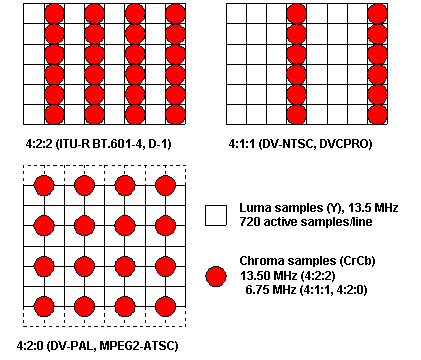
\includegraphics{Image1.png}

\end{multicols}
\end{document}
